%!TEX root = ../template.tex
%% ====================================================================
%% Apêndice A -- Protocolo da revisão e emendas
%% v1 2026-09-16. Substitui o esqueleto de 2026-08-13 (histórico no git).
%% Fontes: protocolo registado (PDF de 2026-02-24), protocolo v2 (abril),
%% LocalResearch/Screening/level3_extraction: OSF_AMENDMENT_DRAFT.md (C-2.3),
%% OSF_AMENDMENT_STAGE_C_DRAFT.md e stage_c/AMENDMENT_FILED.txt (2026-09-13),
%% prisma/PRISMA_FLOW_2026-09-16.md, prisma/PRISMA_ScR_CHECKLIST.md,
%% prisma/SNOWBALLING_NOT_PERFORMED_2026-09-16.md, CORPUS_CLOSURE_2026-09-12.md,
%% AMENDMENT_FN_CENSUS_SAMPLING_2026-09-10.md; calibração das expressões (docx).
%% Decisão de 2026-09-16: não se submetem novas emendas; os desvios posteriores
%% a 2026-09-13 declaram-se apenas aqui.
%% ====================================================================
\chapter{Protocolo da revisão e emendas}
\label{app:protocolo-sr}

Este apêndice documenta o que foi planeado para a revisão de âmbito do Capítulo~\ref{cha:revisao}, quando foi fixado e o que foi executado de outra forma. Reproduz o protocolo tal como foi registado, identifica as três emendas depositadas, apresenta os dados de calibração da pesquisa que o protocolo resume e lista os desvios, incluindo os que não foram objeto de emenda. Termina com a lista de verificação PRISMA-ScR~\cite{Tricco2018}.

\section{Registo e cronologia}
\label{sec:apA-cronologia}

O protocolo foi registado no Open Science Framework a 24 de fevereiro de 2026, com o DOI \nolinkurl{10.17605/OSF.IO/TDW6C}. O registo não antecede a pesquisa nas bases: a calibração das expressões e a execução das pesquisas decorreram em fevereiro de 2026 e o protocolo registado já reporta os volumes recuperados (Secção~4.3 do protocolo). O registo antecede a triagem de título e resumo, a recuperação dos textos integrais, a definição do instrumento de extração e toda a extração: a exportação do Rayyan tem a data do depósito, e a triagem começou depois dele. A Tabela~\ref{tab:apA-cronologia} distingue os registos das etapas de execução que os delimitam.

\begin{table}[H]
\centering\small
\caption{Cronologia dos registos e das etapas de execução da revisão.}
\label{tab:apA-cronologia}
\ntzebra
\begin{tabularx}{\linewidth}{@{}>{\raggedright\arraybackslash}p{2.1cm}>{\raggedright\arraybackslash}X>{\raggedright\arraybackslash}p{3.9cm}@{}}
\toprule
\textbf{Data}  &  \textbf{Registo ou etapa}  &  \textbf{Identificação} \\
\midrule
fev.\ 2026 & \emph{Execução.} Calibração das expressões de pesquisa em cinco configurações e pesquisa na Scopus e na Web of Science (Secção~\ref{sec:apA-pesquisa}). & Documento de calibração; volumes na Secção~4.3 do protocolo \\
2026-02-24 & \emph{Registo.} Protocolo v1.0 (Secção~\ref{sec:apA-protocolo}). & DOI 10.17605/OSF.IO/TDW6C \\
2026-02-24 & \emph{Execução.} Exportação dos registos para o Rayyan: 1\,478 identificados, 925 após deduplicação. & Exportação do Rayyan \\
abr.\ 2026 & \emph{Emenda.} Protocolo v2: clarificação dos dois corpora (Secção~\ref{sec:apA-v2}). & Mesmo registo OSF \\
2026-07-10 & \emph{Execução.} Congelamento dos textos integrais: 459 recuperados de 596 procurados. & Registo de recuperação \\
2026-07-23 & \emph{Emenda.} Protocolo de validação C-2.3: extração assistida por IA e validação humana, antes da extração de produção (Secção~\ref{sec:apA-emendas}). & Projeto OSF \texttt{wh62r}, ficheiro \texttt{6a61e155\allowbreak 18c36790\allowbreak cda322f4}; SHA-256 do PDF \texttt{15c140cd\ldots ec2650} \\
2026-09-12 & \emph{Execução.} Fecho dos corpora: A~=~331, B~=~42. & Registo de fecho do corpus \\
2026-09-13 & \emph{Emenda.} Stage~C: três desvios ao desenho de validação; esquema de extração congelado antes da extração (Secção~\ref{sec:apA-emendas}). & Ficheiro de 59\,079 bytes, SHA-256 \texttt{094fd01a\ldots 9e701}; esquema \texttt{d855254b\ldots e883ff} \\
2026-09-13 a 2026-09-16 & \emph{Execução.} Extração Stage~C sobre o Corpus~B: 41 de 42 publicações; uma em quarentena. & Formulários e dossiês por publicação \\
2026-09-16 & \emph{Desvios não registados.} Retirada da SQ4; rastreio de referências não executado (Secção~\ref{sec:apA-desvios}). & Este apêndice \\
\bottomrule
\end{tabularx}
\end{table}

\section{Protocolo registado}
\label{sec:apA-protocolo}

As páginas seguintes reproduzem o protocolo v1.0 tal como foi registado, em inglês e sem alterações (7 páginas; SHA-256 do ficheiro reproduzido: \texttt{5e30878c\allowbreak 67e54efb\allowbreak 67e6aed7\allowbreak 2c967b37\allowbreak a5ddefbe\allowbreak e5ba8893\allowbreak 676a68a0\allowbreak f99f8a8b}). Contém a pergunta primária, as quatro subquestões, os critérios de elegibilidade no quadro população--conceito--contexto, as duas expressões de pesquisa com a tradução para a Web of Science, o teste de sensibilidade, os três níveis de triagem, o formulário de extração e as limitações antecipadas.

\revisaotese{AP-A-02}{P2}{CONFIRMAR}
{Identidade do PDF reproduzido}
{O PDF foi criado a 2026-02-24 às 15:11 UTC e declara ``Version 1.0 --- registered''. Confirmar no OSF que o hash coincide com o do ficheiro depositado; se não coincidir, substituir pelo descarregado do registo.}

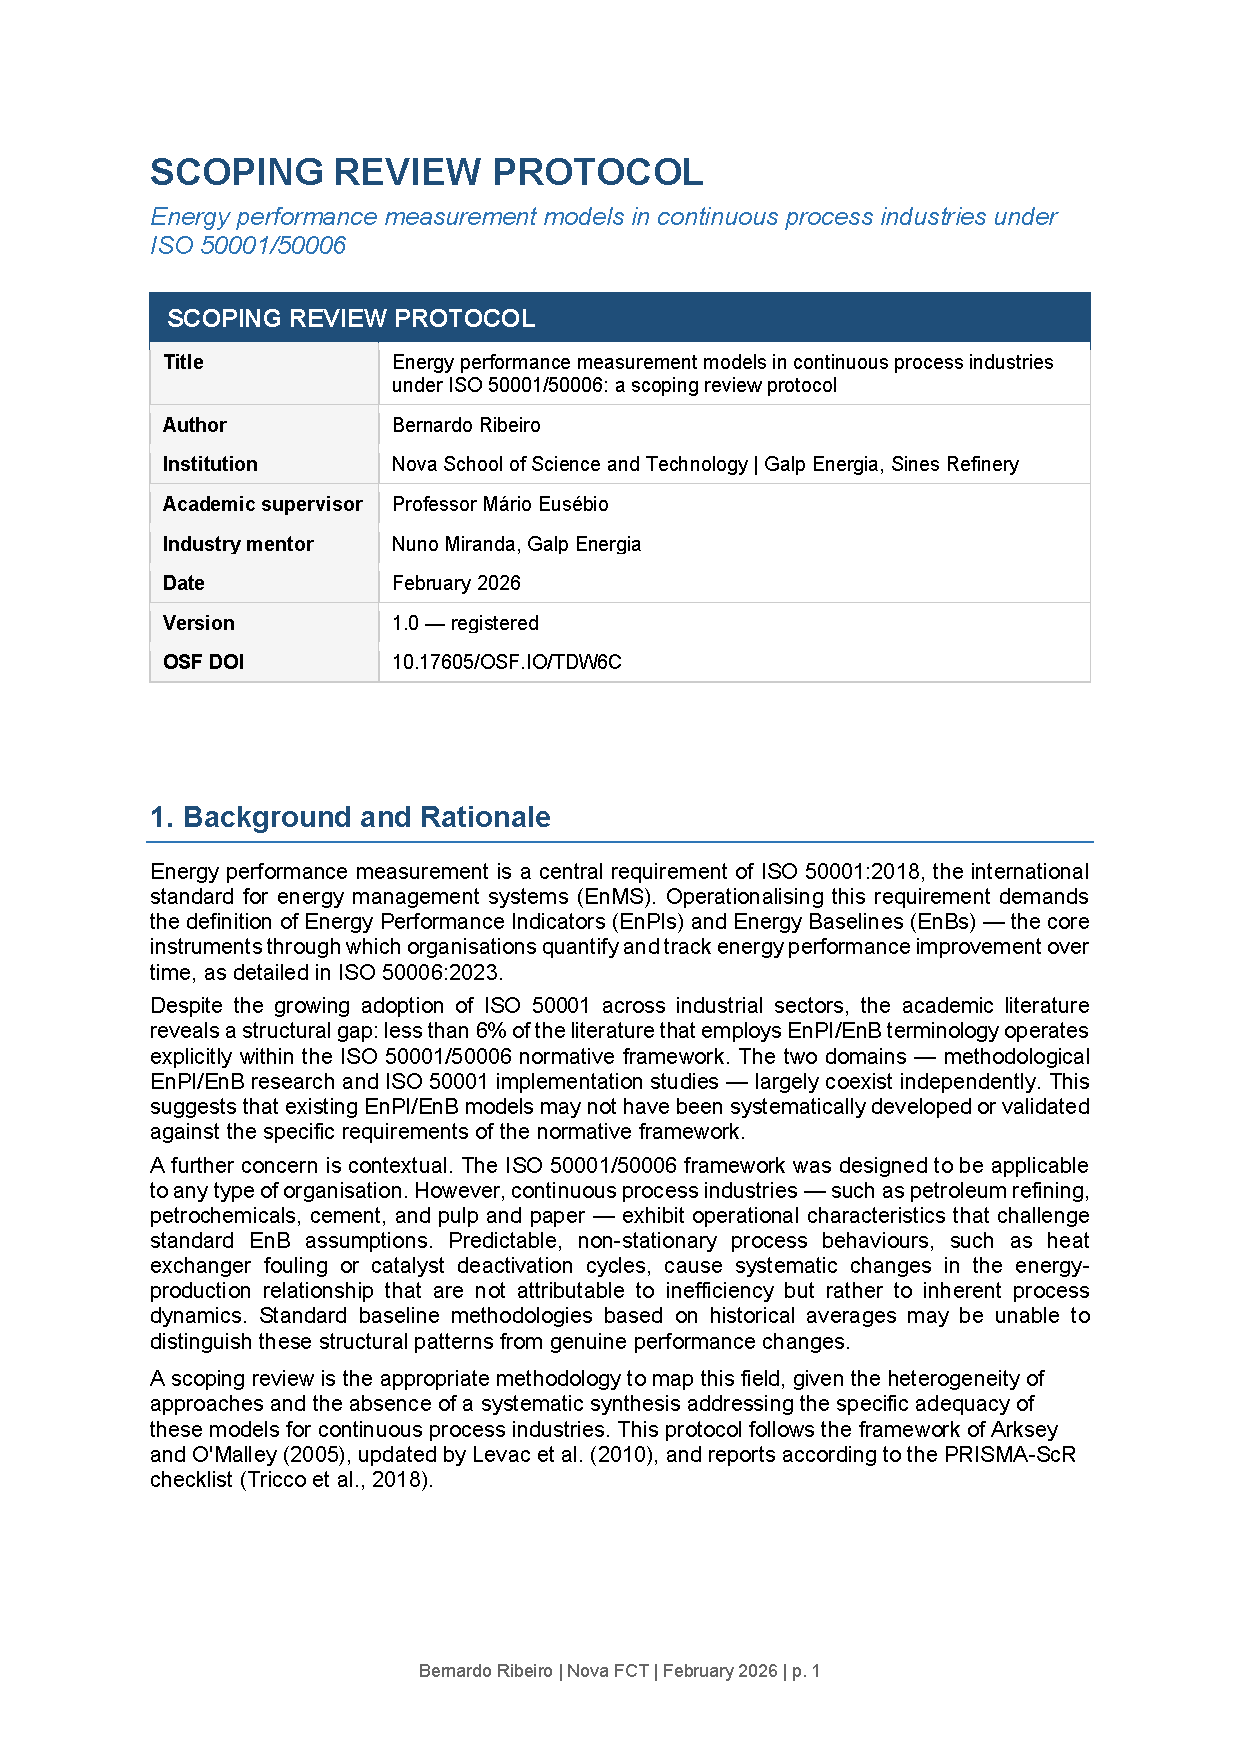
\includepdf[pages=-,scale=0.82,frame,pagecommand={\thispagestyle{plain}}]{5-Figures/apendice-A/protocolo-v1-registado-2026-02-24.pdf}

\section{Emenda de abril de 2026: protocolo v2}
\label{sec:apA-v2}

A emenda de abril tornou explícita a estrutura em dois corpora, que o registo inicial implicava sem a especificar. Declarou não alterar as perguntas, as expressões de pesquisa, os critérios de elegibilidade nem os níveis de triagem. As alterações foram cinco:
\begin{enumerate}[nosep]
  \item Secção~3.1: o Corpus~A reúne todos os registos incluídos, independentemente do setor; o Corpus~B é o subconjunto de A cujo contexto de aplicação é explicitamente uma indústria de processo contínuo.
  \item Secção~5: a avaliação do texto integral passa a aplicar duas determinações sucessivas, a elegibilidade e a classificação no corpus.
  \item Secção~6: as variáveis de nível~A aplicam-se ao Corpus~A e as de nível~B apenas ao Corpus~B.
  \item Secção~7: a análise bibliométrica é atribuída ao Corpus~A e a síntese narrativa ao Corpus~B.
  \item O contexto setorial deixa de constar como critério de exclusão no texto integral e passa a variável de classificação, resolvendo uma inconsistência entre o protocolo registado e o documento de calibração.
\end{enumerate}

\section{Calibração e volumes da pesquisa}
\label{sec:apA-pesquisa}

As expressões finais constam da Secção~4.2 do protocolo reproduzido. A Tabela~\ref{tab:apA-calibracao} regista as cinco configurações testadas em fevereiro de 2026, com acesso pela b-on. As duas adotadas correspondem às expressões A e B do protocolo.

\begin{table}[H]
\centering\small
\caption{Configurações testadas na calibração das expressões de pesquisa (fevereiro de 2026). Volumes antes de deduplicação.}
\label{tab:apA-calibracao}
\ntzebra
\begin{tabularx}{\linewidth}{@{}l>{\raggedright\arraybackslash}Xrrl@{}}
\toprule
\textbf{ID}  &  \textbf{Configuração}  &  \textbf{Scopus}  &  \textbf{WoS}  &  \textbf{Decisão} \\
\midrule
S1/W1 & Bloco EnPI/EnB AND bloco ISO~50001/50006 e sistemas de gestão, com coocorrência obrigatória & 170 & 97 & descartada \\
S2/W2 & Apenas \texttt{"ISO 50001" OR "ISO 50006"} & 468 & 263 & adotada (expressão A) \\
S3/W3 & Apenas o bloco EnPI/EnB, sem contexto; ruído de outros domínios em que ``EnB'' é sigla & 2\,827 & 2\,195 & descartada \\
S4/W4 & ISO~50001/50006 AND termos de desempenho energético & 148 & 79 & descartada \\
S5/W5 & Bloco EnPI/EnB AND bloco de contexto industrial ou de gestão & 486 & 261 & adotada (expressão B) \\
\bottomrule
\end{tabularx}
\end{table}

A S1 foi descartada por perder literatura metodológica que não cita a norma e literatura normativa sem terminologia EnPI/EnB. A S3 tem volume inviável e ruído imediato. O terceiro bloco da S5 mostrou-se mais eficaz do que um filtro por área temática. Com as duas expressões adotadas, a pesquisa identificou 954 registos na Scopus e 524 na Web of Science, 1\,478 no total, reduzidos a 925 após deduplicação no Rayyan. O teste de sensibilidade com cinco artigos âncora recuperou quatro; o quinto, \textcite{Karcher2015}, ficou fora das expressões por não conter metodologia EnPI/EnB, mas entrou na biblioteca pela triagem e foi avaliado em texto integral.

\section{Emendas de julho e de setembro de 2026}
\label{sec:apA-emendas}

\paragraph{Protocolo de validação C-2.3 (2026-07-23).} Depositada antes da extração de produção, esta emenda regista o uso de modelos de linguagem na extração, que o protocolo registado não previa. O revisor único mantém-se como único adjudicador; os modelos são instrumentos de extração e não revisores independentes. A emenda fixou ainda:
\begin{itemize}[nosep]
  \item o âmbito das afirmações: a revisão mapeia o que é reportado na literatura pesquisada, recuperada e elegível, sem matriz de adequação definida \emph{a priori} e sem testar eficácia em Sines;
  \item a lista setorial do Corpus~B, alargada à produção química contínua, aos gases industriais e ao vidro por fusão contínua; casos de fluxo contínuo fora da lista reportam-se à parte como exploratórios;
  \item a interpretação do critério de elegibilidade registado, repondo o limiar original que uma implementação de desenvolvimento tinha tornado mais restritivo;
  \item o desenho de validação humana: adjudicação às cegas das divergências com consequência na pertença aos corpora, controlo de falsos negativos do Corpus~B por união de detetores, cobertura humana do Corpus~B por ramos de dimensão, auditoria por amostragem aleatória simples do nível~A e verificações de ancoragem, de reteste do revisor e de instabilidade dos modelos;
  \item uma regra de suplementação da pesquisa em função do rendimento do rastreio de referências.
\end{itemize}

\paragraph{Emenda Stage~C (2026-09-13).} Depositada antes da extração que governa, declara três desvios ao desenho da C-2.3: (1)~o instrumento de extração do Corpus~B passa a ser o esquema Stage~C (campos C1--C13), e a cobertura humana de 40 publicações às cegas e 2 com pré-preenchimento passa a 11 às cegas e 31 com verificação dos campos que sustentam resultados, ausências incluídas; (2)~a extração decorre numa única superfície de modelo, ficando a segunda família de modelos a rever o instrumento e os registos; (3)~a verificação de ancoragem pode corrigir o localizador de página quando a citação existe palavra por palavra numa única outra página. A emenda declara também que sete veredictos de pertença ao Corpus~B foram adjudicados sobre excertos literais, sem abertura dos PDF completos. O detalhe de cada desvio e as suas consequências para a validação estão no Apêndice~\ref{app:validacao}.

\section{Desvios ao protocolo}
\label{sec:apA-desvios}

A Tabela~\ref{tab:apA-desvios} reúne os desvios ao protocolo e às emendas, registados ou não. Os desvios posteriores a D6 não foram objeto de emenda: por decisão do autor, as alterações posteriores a 13 de setembro de 2026 declaram-se apenas nesta dissertação. Os quatro últimos (D10--D13) são controlos previstos na emenda C-2.3 que não chegaram a ser executados; nenhum deles é invocado no Capítulo~\ref{cha:revisao} como garantia.

{\small
\begin{xltabular}{\linewidth}{@{}l>{\raggedright\arraybackslash}X>{\raggedright\arraybackslash}Xl@{}}
\caption{Desvios ao protocolo registado e às emendas.}\label{tab:apA-desvios}\\
\toprule
\# & Previsto & Executado & Registo \\
\midrule
\endfirsthead
\toprule
\# & Previsto & Executado & Registo \\
\midrule
\endhead
\bottomrule
\endfoot
D1 & Triagem em três níveis sucessivos: título, resumo, texto integral (protocolo, Secção~5). & Título e resumo avaliados na mesma passagem no Rayyan; não há contagens separadas dos dois primeiros níveis. & não registado \\
D2 & Literatura cinzenta de organizações de referência pesquisada nos sítios institucionais (Secção~4.1). & Não pesquisada; a literatura cinzenta ficou limitada ao que as duas bases indexam. & não registado \\
D3 & Extração por revisor humano único com o formulário da Secção~6. & Extração assistida por modelos de linguagem; o revisor adjudica e é responsável pelos registos. & C-2.3 \\
D4 & Extração do Corpus~B por duas famílias de modelos. & Uma superfície de modelo no Stage~C. & 2026-09-13 \\
D5 & Localizador de página fixado pela superfície de extração. & Corrigível pela verificação de ancoragem quando a citação existe numa única outra página. & 2026-09-13 \\
D6 & Controlo de falsos negativos do Corpus~B com decisão humana fundamentada por candidato (C-2.3). & A primeira passagem, de 2026-09-10, produziu 171 de 177 veredictos sem leitura, que foram anulados e preservados fora de qualquer cálculo. O fecho de 2026-09-12 incluiu uma passagem exaustiva sobre um subconjunto de risco definido deterministicamente (5 publicações) e sete veredictos adjudicados sobre excertos. Falsos negativos confirmados: zero. & parcial (2026-09-13) \\
D7 & Cobertura humana do Corpus~B: 11 publicações às cegas e 31 com verificação dos campos que sustentam resultados (emenda de 2026-09-13). & Não executada como previsto. Os registos Stage~C têm verificação automática de ancoragem das citações ao texto. A 2026-09-17, as 368 células com citação que sustentam resultados foram relidas por um segundo passe de modelo da mesma família do extrator, com regra de adjudicação fixa; 31 células e duas regras ficaram para decisão do autor e uma amostra de dez confirmações para leitura humana (Apêndice~\ref{app:validacao}). As ausências não foram verificadas. & não registado \\
D8 & Subquestão SQ4, sobre aplicabilidade na refinação (protocolo e emendas). & Retirada a 2026-09-16: sem a leitura às cegas das 11 publicações nucleares, a revisão não sustenta afirmações de transferibilidade para a refinação. & não registado \\
D9 & Rastreio de referências retrospetivo e prospetivo, com regra de suplementação da pesquisa (Secções~4.1 e~5; C-2.3). & Não executado, por decisão de 2026-09-16. O rendimento é nulo por omissão e não por resultado; o custo foi estimado e é declarado como limitação no Capítulo~\ref{cha:revisao}. & não registado \\
D10 & Auditoria por amostragem das decisões de elegibilidade do nível~A, com 40 registos e semente 44 (C-2.3). & Não executada. Não há registo da corrida, e um controlo que a dissertação declarasse ter feito sem o poder mostrar valeria menos do que a sua ausência declarada. & não registado \\
D11 & Reteste de 30 decisões do revisor, para medir concordância intra-revisor (C-2.3). & Não executado, pela mesma razão. A verificação do Corpus~B (D7) cobre a extração, não a triagem. & não registado \\
D12 & Canário de instabilidade em 30 publicações, para detetar deriva entre lotes (C-2.3). & Não executado. A estabilidade entre lotes não foi medida; as contagens do Capítulo~\ref{cha:revisao} devem ler-se sem esse controlo. & não registado \\
D13 & Pesquisa terminológica nas exclusões de título e resumo, com amostra de 50 (C-2.3). & Não executada. É o controlo cuja ausência mais pesa: os falsos negativos da triagem ficam sem estimativa própria, e só o rastreio de referências (D9), também não executado, os apanharia. & não registado \\
D14 & Análise por expressão de pesquisa: atribuir cada registo à expressão~A, à~B ou a ambas, para medir o rendimento de cada uma. & Não executada. O campo de origem ficou vazio no ficheiro analítico e um valor vazio não distingue «entrou por rastreio» de «não foi registado»; recuperá-lo obrigaria a voltar aos ficheiros de exportação das bases. Nenhuma conclusão da revisão depende desta análise. & não registado \\
D15 & O protocolo não especifica como se decide que duas extrações dão o mesmo valor; na C-2.3 a concordância entre modelos é um sinal de encaminhamento do esforço humano, não uma métrica. & A comparação é feita sobre a forma normalizada dos campos em texto livre, com o vocabulário controlado que serve a derivação, e não sobre a resposta em bruto. A regra foi alterada a 2026-09-21, depois de os resultados do Capítulo~\ref{cha:revisao} estarem escritos: o setor passou de 145 para 201 classificações concordantes e o país de 144 para 178; os restantes oito campos não se alteraram. Não introduz vocabulário novo nem adjudicação humana. & não registado \\
\end{xltabular}
}

\section{Lista de verificação PRISMA-ScR}
\label{sec:apA-prisma}

A Tabela~\ref{tab:apA-prisma} indica onde cada item da extensão PRISMA-ScR~\cite{Tricco2018} é tratado nesta dissertação. A revisão é um capítulo e não um relato autónomo, pelo que os itens de título e resumo se aplicam com adaptação.

{\small
\begin{xltabular}{\linewidth}{@{}r>{\raggedright\arraybackslash}p{3.3cm}>{\raggedright\arraybackslash}p{3.6cm}>{\raggedright\arraybackslash}X@{}}
\caption{Lista de verificação PRISMA-ScR.}\label{tab:apA-prisma}\\
\toprule
\# & Item & Onde & Nota \\
\midrule
\endfirsthead
\toprule
\# & Item & Onde & Nota \\
\midrule
\endhead
\bottomrule
\endfoot
\multicolumn{4}{@{}l}{\emph{Título e resumo}}\\
1 & Título & Capítulo~\ref{cha:revisao} & O capítulo identifica-se como revisão de âmbito. \\
2 & Resumo estruturado & Resumo & Adaptado: o resumo da dissertação refere a revisão e a extração assistida por IA. \\
\multicolumn{4}{@{}l}{\emph{Introdução}}\\
3 & Fundamentação & Secções~\ref{sec:problema} e~\ref{sec:protocolo-sr} & \\
4 & Objetivos & Secções~\ref{sec:objetivos} e~\ref{sec:protocolo-sr} & SQ4 registada e retirada (desvio D8). \\
\multicolumn{4}{@{}l}{\emph{Métodos}}\\
5 & Protocolo e registo & Secções~\ref{sec:protocolo-sr} e~\ref{sec:apA-cronologia} & DOI 10.17605/OSF.IO/TDW6C; registo a 2026-02-24; três emendas. \\
6 & Critérios de elegibilidade & Secções~\ref{sec:pesquisa} e~\ref{sec:apA-protocolo} & Com a clarificação da Secção~\ref{sec:apA-v2}. \\
7 & Fontes de informação & Secções~\ref{sec:pesquisa} e~\ref{sec:apA-pesquisa} & Scopus e Web of Science, via b-on; fevereiro de 2026. \\
8 & Pesquisa & Secções~\ref{sec:apA-protocolo} e~\ref{sec:apA-pesquisa} & Expressões completas na Secção~4.2 do protocolo reproduzido. \\
9 & Seleção das fontes & Secção~\ref{sec:pesquisa} & Revisor único; desvio D1. \\
10 & Extração dos dados & Secção~\ref{sec:pesquisa}; Apêndice~\ref{app:validacao} & Assistida por IA; desvios D3--D7; Declaração de uso de IA. \\
11 & Itens extraídos & Apêndice~\ref{app:validacao} & Nível~A no Corpus~A; campos C1--C13 no Corpus~B. \\
12 & Avaliação crítica das fontes & --- & Não realizada, como é próprio de uma revisão de âmbito~\cite{Arksey2005,Levac2010}. \\
13 & Síntese & Secções~\ref{sec:corpus-a} e~\ref{sec:corpus-b} & Distribuição descritiva (SQ1) e síntese narrativa (SQ2--SQ3), sem meta-análise. \\
\multicolumn{4}{@{}l}{\emph{Resultados}}\\
14 & Seleção das fontes & Secção~\ref{sec:pesquisa} & Fluxograma sem caixa de rastreio de referências (desvio D9). \\
15 & Características das fontes & Secção~\ref{sec:corpus-a} & \\
16 & Avaliação crítica nas fontes & --- & Não aplicável (item~12). \\
17 & Resultados por fonte & Apêndice~\ref{app:validacao} & Formulários e dossiês das 41 publicações extraídas, com citações ancoradas à página, em material suplementar. \\
18 & Síntese dos resultados & Secções~\ref{sec:corpus-a} e~\ref{sec:corpus-b} & \\
\multicolumn{4}{@{}l}{\emph{Discussão}}\\
19 & Sumário da evidência & Secção~\ref{sec:gap} & \\
20 & Limitações & Secções~\ref{sec:gap} e~\ref{sec:limitacoes} & Revisor único; 137 textos não recuperados, de forma não aleatória; extração numa superfície de IA sem verificação humana por ocorrência; só inglês; literatura cinzenta parcial; SQ4 retirada; rastreio de referências não executado. \\
21 & Conclusões & Secção~\ref{sec:gap}; Capítulo~\ref{cha:conclusoes} & \\
\multicolumn{4}{@{}l}{\emph{Financiamento}}\\
22 & Financiamento & Este apêndice & A revisão não teve financiamento específico. O autor realizou estágio curricular na organização que é objeto do caso empírico dos Capítulos~\ref{cha:plataforma} e~\ref{cha:diagnostico}, e suportou os custos de computação da extração. \\
\end{xltabular}
}

